% !TEX TS-program = pdflatex
% !TEX encoding = UTF-8 Unicode

% This is a simple template for a LaTeX document using the "article" class.
% See "book", "report", "letter" for other types of document.

\documentclass[11pt]{article} % use larger type; default would be 10pt

\usepackage[utf8]{inputenc} % set input encoding (not needed with XeLaTeX)

%%% Examples of Article customizations
% These packages are optional, depending whether you want the features they provide.
% See the LaTeX Companion or other references for full information.

%%% PAGE DIMENSIONS
\usepackage{geometry} % to change the page dimensions
\geometry{a4paper} % or letterpaper (US) or a5paper or....
\geometry{margin=1in} % for example, change the margins to 2 inches all round
% \geometry{landscape} % set up the page for landscape
%   read geometry.pdf for detailed page layout information

\usepackage{graphicx} % support the \includegraphics command and options

% \usepackage[parfill]{parskip} % Activate to begin paragraphs with an empty line rather than an indent
\usepackage{amssymb}
\usepackage{amsmath}
%%% PACKAGES
\usepackage{booktabs} % for much better looking tables
\usepackage{array} % for better arrays (eg matrices) in maths
\usepackage{paralist} % very flexible & customisable lists (eg. enumerate/itemize, etc.)
\usepackage{verbatim} % adds environment for commenting out blocks of text & for better verbatim
\usepackage{subfig} % make it possible to include more than one captioned figure/table in a single float
% These packages are all incorporated in the memoir class to one degree or another...

%%% HEADERS & FOOTERS
\usepackage{fancyhdr} % This should be set AFTER setting up the page geometry
\pagestyle{fancy} % options: empty , plain , fancy
\renewcommand{\headrulewidth}{0pt} % customise the layout...
\lhead{}\chead{}\rhead{}
\lfoot{}\cfoot{\thepage}\rfoot{}

%%% SECTION TITLE APPEARANCE
\usepackage{sectsty}
\allsectionsfont{\sffamily\mdseries\upshape} % (See the fntguide.pdf for font help)
% (This matches ConTeXt defaults)

%%% ToC (table of contents) APPEARANCE
\usepackage[nottoc,notlof,notlot]{tocbibind} % Put the bibliography in the ToC
\usepackage[titles,subfigure]{tocloft} % Alter the style of the Table of Contents
\usepackage{bbm}
\usepackage{endnotes}

\renewcommand{\cftsecfont}{\rmfamily\mdseries\upshape}
\renewcommand{\cftsecpagefont}{\rmfamily\mdseries\upshape} % No bold!
\DeclareMathOperator*{\argmax}{arg\,max}
\DeclareMathOperator*{\argmin}{arg\,min}

\usepackage{graphicx}
\graphicspath{ {./pings/} }

\newcount\colveccount
\newcommand*\colvec[1]{
        \global\colveccount#1
        \begin{pmatrix}
        \colvecnext
}
\def\colvecnext#1{
        #1
        \global\advance\colveccount-1
        \ifnum\colveccount>0
                \\
                \expandafter\colvecnext
        \else
                \end{pmatrix}
        \fi
}

\newcommand{\norm}[1]{\left\lVert#1\right\rVert}

\title{Econometrics HW5}
\author{Michael B. Nattinger\footnote{I worked on this assignment with my study group: Alex von Hafften, Andrew Smith, and Ryan Mather. I have also discussed problem(s) with Emily Case, Sarah Bass, Katherine Kwok, and Danny Edgel.}}

\begin{document}
\maketitle

\section{Question 25.1}
The estimated probabilities of purchase and not purchase will be the same across the two models, so we can write the probabilities as follows:
\begin{align*}
P(\text{purchase}|X=x) &= 1-P(\text{no purchase}|X=x)\\
\Phi(x'\beta_1) &= 1-\Phi(x'\beta_2)\\
&= \Phi(-x'\beta_2)\\
\Rightarrow \beta_1 &= -\beta_2.
\end{align*}
\section{Question 25.3}
Let $Y = P(X) + e$ and note that $Y = \begin{cases} 1, \text{ w.p. } P(X) \\ 0, \text{ w.p. } 1-P(X)\end{cases}$.\\ Solving for $e$ we have $e = \begin{cases} 1-P(X), \text{ w.p. } P(X) \\ -P(X), \text{ w.p. } 1-P(X)\end{cases}$. It is trivial to see that $E[e|X] = 0$.

\begin{align*}
E[e^2|X] &= (1-P(X))^2P(X) + (-P(X))^2(1-P(X)) \\
&= (1-2P(X) + P(X)^2)P(X) + P(X)^2 - P(X)^3\\
&= P(X) - P(X)^2\\
&= P(X)(1-P(X)),\\
\Rightarrow Var(e|X) &= P(X)(1-P(X)).
\end{align*}
\section{Question 25.9}
From (25.5), the conditional probability mass function is
\begin{align*}
\pi(Y|X) &= \Lambda(Z'\beta)\\
&= (1+exp(-Z'\beta))^{-1},
\end{align*}
where $Z = \begin{cases} X, \text{ if } Y=1 \\ -X, \text{ if } Y=0 \end{cases}$. Given data we can write the log likelihood function as the following:
\begin{align*}
L(\beta) &= \sum_{i=1}^n log((1+exp(-Z_i'\beta))^{-1}) \\\
&= -\sum_{i=1}^n log(1+exp(-Z_i'\beta))
\end{align*}
Taking FOCs of the log likelihood function,
\begin{align*}
\sum_{i=1}^n (1+exp(-Z_i'\beta))^{-1}exp(-Z_i'\beta)Z_i &= \vec{0}\\
\sum_{i=1}^n (1-\Lambda(Z_i\beta))Z_i &= \vec{0}
\end{align*}
Then, $\hat{\beta}_{MLE}$ is the solution to this set of equations. Note that this solution has no closed form.
\section{Question 25.12}
Given data, the NLLS estimator would minimize the sum of square errors:
\begin{align*}
\hat{\beta}_{NLLS} &= \argmin_{\beta} \sum_{i=1}^n (Y_i - \Lambda(X_i \beta))^2
\end{align*}
\section{Question 25.14}
\subsection{Part A}
\begin{align*}
P(Y>0) &= P(Y^{*}>0)\\
&= P(m(X) + e >0)\\
&= P(e>-m(X))\\
&= 1-\Phi_{\sigma^2(X)}(-m(X))
\end{align*}
where $\Phi_{\sigma^2(X)}$ is the CDF of $N(0,\sigma^2(X))$.
\subsection{Part B}
No. Assume for the purpose of contradiction that $m(X)$ and $\sigma^2(X)$ were uniquely identified. Then, note that $m'(X) = cm(X), \sigma^{2'}(X) = c^2\sigma^2(X)$  yield the same response probability so the identification is not unique.
\subsection{Part C}
Normalize $\sigma^2(X) = 1.$ Then we can identify $\tilde{m}(X)$, which is the $m$ function transformed appropriately s.t. the normalization of $e$.
\subsection{Part D}
No, $\sigma^2(X) = 1 \forall X$ so there is no heteroskedasticity in the model.
\section{Question 25.15} 

Below are the estimated coefficients.

\begin{center}
\begin{tabular}{ll}
& Equilibrium \\ 
\hline 
Capital & 5.0451 \\ 
Wage & 1.1461 \\ 
Interest rate & 0.12778 \\ 
\hline 
\end{tabular}
\end{center}

From the coefficients and standard errors which we were asked to provide, we can see that age, education, and the indicator for hispanic are significant coefficients in the logit model we were asked to run. Note that the marginal effect is not directly seen in the information we were asked to provide. 

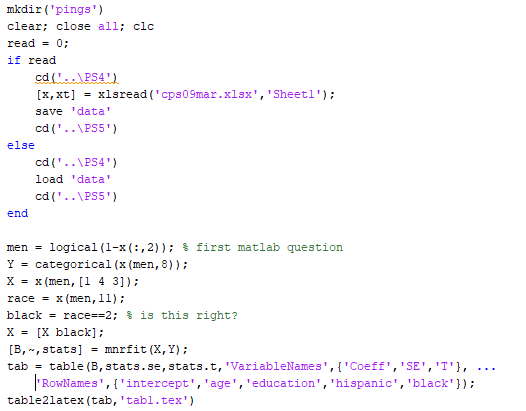
\includegraphics{p1}

\section{Question 25.17} %stata

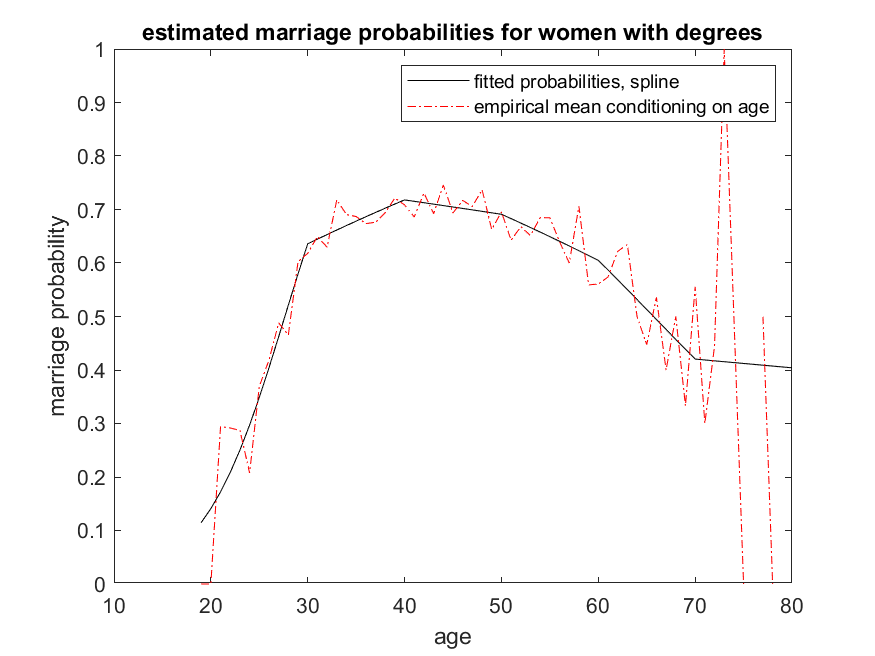
\includegraphics{fig1}

Above we see the results for the model that I decided on. I included linear splines for age above 30, 40, 50, 60, and 70. To visually check the model results, I estimated the mean of the marriage indicator at each age. This is plotted on the figure in the red dashed line. From comparing the fitted logit model to the nonparametric conditional estimate we can see that the model appears to fit the data reasonably well.

My reasoning for the linear splines at decade intervals was an intuition that each decade of life may, for a variety of reasons, lead to different relationships between age and marriage. I used a linear spline rather than a quadratic spline as the number of knots on the spline was 5, which already seemed fairly large and so I did not want to include the extra quadratic terms. Additionally, the splines seemed to fit the data well from just the linear terms. 

Comparing to figure 25.1, it is clear that the marriage probabilities are lower for educated women than men. Moreover, for educated women there appears to be a significant drop-off in marriage probabilities after around the age of 60. This does not appear in the distribution of men. If anything, the distribution of men appears to begin to rise after 60.

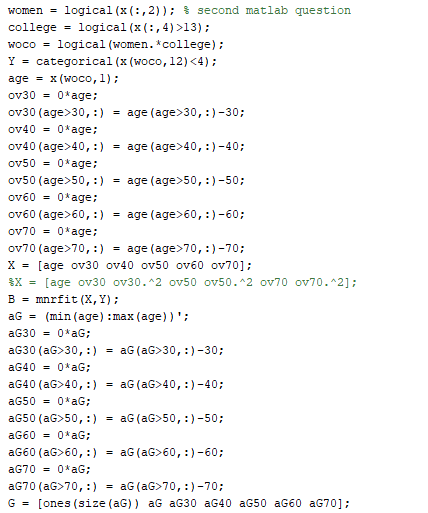
\includegraphics{p2}

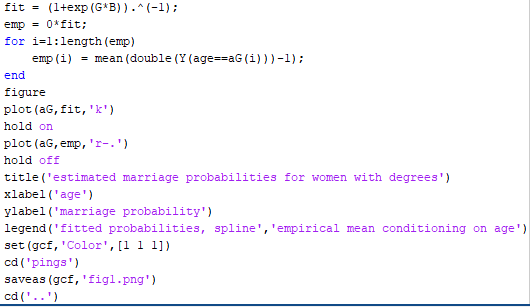
\includegraphics{p3}

\section{Question 26.1}
\begin{align*}
P_j(x) &= \frac{exp(x'\beta_j)}{\sum_{l=1}^{J}exp(x'\beta_l)}.\\
exp(a) &> 0\\
\Rightarrow P_j(x) &>0.\\
\frac{exp(x'\beta_j)}{\sum_{l=1}^{J}exp(x'\beta_l)} &< \frac{exp(x'\beta_j)}{exp(x'\beta_j)}\\
&= 1.\\
\Rightarrow 0\leq P_j(x)&\leq 1\\.
\sum_{j=1}^J P_j(x) &= \sum_{j=1}^J \frac{exp(x'\beta_j)}{\sum_{l=1}^{J}exp(x'\beta_l)}\\
&= \frac{\sum_{j=1}^{J}exp(x'\beta_j)}{\sum_{l=1}^{J}exp(x'\beta_l)}\\
&=1.
\end{align*}
\section{Question 26.3}
\begin{align*}
\frac{\partial P_j(x)}{\partial x} &= \frac{\partial }{\partial x} \frac{exp(x'\beta_j)}{\sum_{l=1}^{J}exp(x'\beta_l)}\\
&=  \frac{exp(x'\beta_j)}{\sum_{l=1}^{J}exp(x'\beta_l)} \beta_j -  \frac{exp(x'\beta_j)}{\sum_{l=1}^{J}exp(x'\beta_l)} \frac{\sum_{i=1}^J(exp(x'\beta_i)\beta_i)}{\sum_{l=1}^{J}exp(x'\beta_l)}\\
&= P_j(x)\left(\beta_j - \sum_{i=1}^J P_{i}\beta_i \right)
\end{align*}
\section{Question 26.7}
The average marginal effects can be written in the following form:
\begin{align*}
AME_{jj} &= E[\delta_{jj}(W,X)]\\
&= E[\gamma P_{j}(W,X)(1-P_j(W,X))]
\end{align*}
Replacing expectations with sample averages and estimated coefficients and probabilities, we get the following:
\begin{align*}
\hat{AME}_{jj} &= \hat{\gamma}\frac{1}{n}\sum_{i=1}^n\hat{P}_j(W_i,X_i)(1-\hat{P}_j(W_i,X_i)).
\end{align*}
\section{Question 26.8}
For a multinomial logit model we have the following:
\begin{align*}
\frac{P_j(W,X|\theta)}{P_l(W,X|\theta)} &= \frac{\frac{exp(W'\beta_j + X_j'\gamma)}{\sum_{i=1}^{J}exp(W'\beta_i + X_i'\gamma)}}{\frac{exp(W'\beta_l + X_l'\gamma)}{\sum_{i=1}^{J}exp(W'\beta_i + X_i'\gamma)}} \\
&= \frac{exp(W'\beta_j + X_j'\gamma)}{exp(W'\beta_l + X_l'\gamma)}.
\end{align*}

\end{document}
